
\documentclass[report,11pt]{article} 

\usepackage[english]{babel}
\usepackage[utf8]{inputenc}
\usepackage{amsmath,amssymb}
\usepackage{graphicx}
\usepackage{tikz}
\usetikzlibrary{shapes}
\usepackage{natbib}
\usepackage{hyperref}


\title{
{Thesis Title}\\
{\large Institution Name}\\

\hfill

{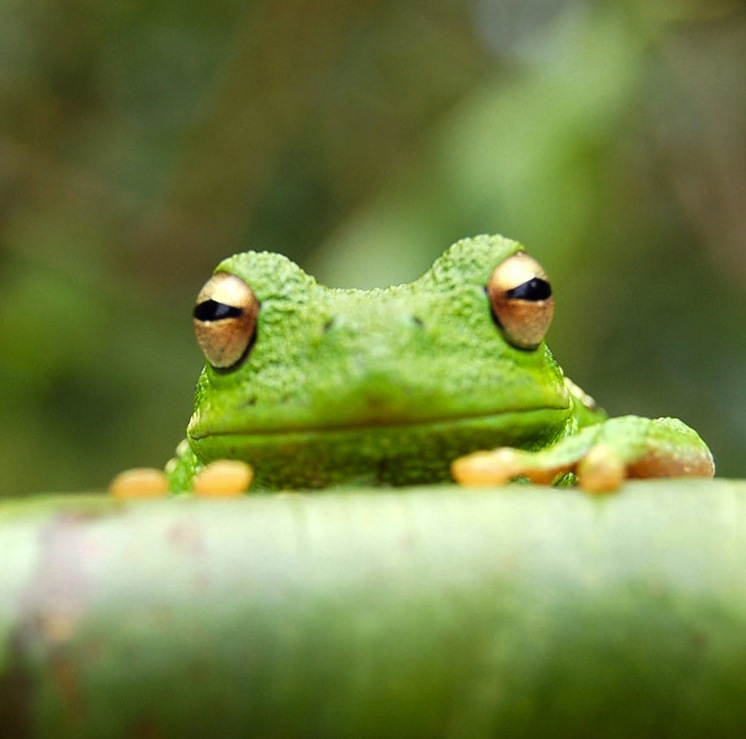
\includegraphics[width=0.3\textwidth]{frog}}

\author{Author Name}
\date{Day Month Year}
}
\begin{document}
\pagenumbering{gobble} 
\maketitle

\newpage

\input{front_matter/title_page.tex}

\tableofcontents
\newpage




\begin{abstract}
\thispagestyle{plain}
\begin{center}
    \Large
    \textbf{Thesis Title}
        
    \vspace{0.4cm}
    \large
    Thesis Subtitle
        
    \vspace{0.4cm}
    \textbf{Author Name}
       
    \vspace{0.9cm}
    \textbf{Abstract}
\end{center}
Lorem ipsum dolor...
\end{abstract}

 \section{Introduction}

\LaTeX{} is great at typesetting mathematics. Let $X_1, X_2, \ldots, X_n$ be a sequence of independent and identically distributed random variables with $\text{E}[X_i] = \mu$ and $\text{Var}[X_i] = \sigma^2 < \infty$, and let
$$S_n = \frac{X_1 + X_2 + \cdots + X_n}{n}
      = \frac{1}{n}\sum_{i}^{n} X_i$$
denote their mean. Then as $n$ approaches infinity, the random variables $\sqrt{n}(S_n - \mu)$ converge in distribution to a normal $\mathcal{N}(0, \sigma^2)$.
\newpage

%%%%%%%%%%%%%%%%%% SECTION 2 %%%%%%%%%%%%%%%%%%
\section{Literature review} % edit section heading as appropriate
    \subsection{Introduction}
	
	
	\subsection{Detail}

	\subsection{More detail}
	\subsection{Summary}


%%%%%%%%%%%%%%%%%% SECTION 3 %%%%%%%%%%%%%%%%%%
\section{Methods} % edit section heading as appropriate
    \subsection{Introduction}
	
	\subsection{Detail}
   
	\subsection{More detail}
	
	
	\subsection{Summary}
	

%%%%%%%%%%%%%%%%%% SECTION 4 %%%%%%%%%%%%%%%%%%
\section{Results and discussion} % edit section heading as appropriate
    \subsection{Introduction}
	
	\subsection{Detail}
 
	\subsection{More detail}
	
	\subsection{Summary}
	
% Add more sections if necessary


%%%%%%%%%%%%%%%%%% SECTION 5 %%%%%%%%%%%%%%%%%%
\section{Conclusions and future work} % edit section heading as appropriate
    \subsection{Conclusions}

	\subsection{Future work}

\bibliographystyle{unsrt}
%\bibliography{references}

\end{document}